\chapter{\IfLanguageName{dutch}{Implementatie}{Implementation}}
\label{ch:implementatie}

Aan de hand van de RPA provider UiPath zullen enkele concrete processen geautomatiseerd worden op Metamaze, het automated document processing platform bij Faktion zelf.

\section{De tools}
Na het afwerken van de cursus 'RPA developer essentials training', aangeboden op de site van UiPath\footnote{\url{https://academy.uipath.com/}} zelf, zal ook de UiPath software suite gebruikt worden om de processen uit te werken. Deze tool suite bestaat uit 3 grote delen:

\subsection{UiPath Studio}
Deze omgeving staat toe om automatisatie workflows visueel, snel en met een beperkte programmeer kennis op te bouwen. Studio is waar de geautomatiseerde processen gebouwd worden in een visuele manier. Hiervoor kan gebruik gemaakt worden van de ingebouwde recorder, drag \& drop van activiteiten en best-practice templates.

\subsection{UiPath Orchestrator}
De orchestrator wordt gebruikt om de verschillende robots te gaan deployen, onderhouden en minotoren. Het is ook de plek waar libraries, herbruikbare componenten, assets en processen die gebruikt worden door deze robots opgeslagen zijn.

De orchestrator is een server gebaseerde applicatie die beschikbaar is via de browser, waarlangs de robotische werkkracht gecontrolleerd, onderhouden en gemonitord wordt:
\begin{itemize}
	\item De connecties met de robot worden gemaakt en onderhouden, de robotten worden gegroepeerd (controle).
	\item De geautomatiseerde processen worden verspreid als taken voor de robot (management)
	\item De uitvoer van een taak wordt genoteerd en bijgehouden (monitoring)
\end{itemize}

\subsection{De robot}
De robot is degene die de workflow en instructies die het ontvangt gaat uitvoeren. Hierbij zijn er twee types.

\subsubsection{Attended}
De robot wordt geactiveerd door gebruiker input en werkt onder supervisie van een werknemer op hetzelfde werkstation.

\subsubsection{Unattended}
De robot werkt in een virtuele werkomgeving zonder toezicht van een werknemer en kan eender welk nummer van processen uitvoeren.

\section{Een proces}
Een proces is een verzameling van activiteiten die input omzetten naar output. Algemeen kan gesteld worden dat de output van het ene proces de input is van de volgende.

[enkele termen]

\subsection{De relatie tussen een proces en een procedure}
Er zijn vele elementen die niet vernoemd worden in de definitie van een standaard proces zoals tijd beperkingen, afhankelijkheid van andere processen en variaties over hoe resources toegekend worden. Dit is waar procedures helpen. Een procedure vult extra informatie aan over een proces en beschrijft hoe het uitgevoerd moet worden, wie verantwoordelijk is voor elk deel van het proces, wanneer elk deel moet uitgevoerd worden, hoe er best wordt omgegaan met uitzonderingen en de specificaties die toepasbaar zijn op ieder deel.

\subsection{Wat maakt een proces een goede kandidaat voor automatisatie}
Er zijn een aantal factoren waarmee rekening gehouden moet worden bij het overwegen of een proces geschikt is voor automatisering. Normaal worden de analyse en prioriteitsstelling uitgevoerd door een RPA Business Analist (BA), maar het is handig voor ontwikkelaars om deze ook te evalueren aangezien bij kleinere implementaties misschien geen BA nodig is in het team. Er zijn twee criteria die u kunt gebruiken om het automatiseringspotentieel te bepalen: de fitheid van een proces en de complexiteit van automatisering.

\subsection{Process Fitness}
Dit zijn de criteria die gebruikt kunnen worden om:
\begin{itemize}
	\item Rule based: de beslissingen (inclusief gegevensinterpretatie) in het proces kunnen worden vastgelegd in een vooraf gedefinieerde logica. Het uitzonderingspercentage is laag of kan mee worden opgenomen in de bedrijfslogica.
	\item Automatable and/or repetitive tasks: we kunnen 4 soorten processen onderscheiden:
		\subitem Manual \& non-repetitive: de stappen in het proces worden uitgevoerd door mensen en zijn elke keer anders.
		\subitem  Manual \& repetitive: de stappen in het proces worden uitgevoerd door mensen. Sommige stappen blijven hetzelfde.
		\subitem  Semi-automated \& repetitive: enkele zijn al geautomatiseerd via Excel en macro's
		\subitem  Automated: er zijn processen die reeds geautomatiseerd zijn door technologieën zoals RPA.
		Processen die handmatig moeten blijven, niet-repetitief zijn vanwege het hoge aantal uitzonderingen of factoren die niet in een bedrijfslogica kunnen worden geïntegreerd, zijn geen goede kandidaten voor automatisering.
		\item Standard input: De input in het proces moet elektronisch zijn en gemakkelijk leesbaar of leesbaar met behulp van een technologie die kan worden geassocieerd met RPA (zoals OCR). Een goed voorbeeld is een factuur met vooraf gedefinieerde velden.
		\item Stable: processen die al lange tijd geen wijzigingen gehad hebben en waarbij er ook geen verwacht worden in de komende maanden zjin goede kandidaten voor automatisering, gegeven dat ze de andere criteria ook voldoen.
\end{itemize}

\subsection{Automatie Complexiteit}
Deze verzameling van criteria bepaalt de moeilijkheidsgraad om een proces te automatiseren:

\begin{itemize}
	\item Aantal schermen: RPA werkt door de robot te programmeren om taken op schermniveau uit te voeren (wanneer het scherm verandert, moet de logica worden aangeleerd). Hoe hoger het aantal schermen, hoe meer elementen moeten worden vastgelegd en geconfigureerd voorafgaand aan de procesautomatisering.
	\item Types van applicaties: sommige applicaties zijn eenvoudiger te automatiseren (zoals de Office-suite of browsers), andere verhogen de automatisering aanzienlijk (bijvoorbeeld Mainframe).
	\item Bedrijfslogica scenario's: de complexiteit van een automatisering neemt toe met het aantal beslissingspunten in de bedrijfslogica. In principe zou elk punt het aantal scenario's met twee kunnen vermenigvuldigen.
	\item Typen en aantal inputs: Standaardinvoer is wenselijk. Toch zijn er gevallen waarin voor elke leverancier een standaardinvoer (zoals een factuur) moet worden geconfigureerd die door de automatisering wordt beïnvloed. Bovendien kan niet-standaard invoer verschillende complexiteitsgraden hebben, waarbij vrije tekst het meest complex is.
\end{itemize}

Gebruik makende van de vorige criteria kunnen categorieën onderscheiden worden:
\begin{itemize}
	\item Geen RPA: processen die frequent veranderen, de systeemomgeving vluchtig is en meerdere handmatige (zelfs niet-digitale) acties vereist zijn
	\item Semi-automatisering: processen die kunnen worden onderverdeeld in stappen die duidelijk kunnen worden geautomatiseerd, en stappen die handmatig moeten blijven (zoals validaties of gebruik van fysieke beveiligingstokens)
	\item High-cost RPA: processen die digitaal zijn en kunnen worden geautomatiseerd, maar gebruik maken van een aantal complexe technologieën (zoals OCR) of geavanceerde programmeervaardigheden vereisen.
	\item Zero-Touch automation: processen die digitaal zijn en betrekking hebben op een zeer statisch systeem, zodat ze gemakkelijk kunnen worden onderverdeeld in instructies en zodat eenvoudige triggers kunnen worden gedefinieerd.
\end{itemize}

\section{Verschillende rollen binnen een RPA oplossing}

\subsection{Solution Architect}
Heeft de leiding over de architectuur van de RPA-oplossing. De Solution Architect vertaalt de vereisten van de functionele analisten en creëert de architectuur- en ontwerpartefacten. Ze leiden, adviseren en zijn verantwoordelijk voor de teamlevering van de ontwikkelaars.

\subsection{Business Analist}
Is verantwoordelijk voor het in kaart brengen van de 'AS IS' en voorgestelde 'TO BE' processen. Businessanalisten hebben kennis van het bedrijfsproces dat geautomatiseerd wordt, algemene bedrijfsprocestheorie en RPA-mogelijkheden. Ze zijn verantwoordelijk voor het vermelden van de procesvereisten nodig voor automatisering, het verduidelijken van de inputs en verwachte outputs en het creëren van RPA-documenten (procesontwerpdocumenten, proceskaarten).

\subsection{Project Manager}
Vormt en beheert het RPA-team, doet resourceplanning en beschikbaarheid van het team om de automatiseringsdoelen te halen. Meestal is de PM de Single Point of Contact (SPOC) voor vragen, RPA-initiatieven of parallelle RPA-productprojecten.

\subsection{RPA Developer}
Bij complexe projecten zullen verschillende ontwikkelaars samenwerken om alle processen te automatiseren.

\subsection{IT security}
Met goede technische en beveiligingsvaardigheden zijn ze verantwoordelijk voor het instellen en onderhouden van hardware- \& softwarebronnen. Ze zetten accounts op voor alle ontwikkelaars, eindgebruikers en robots.

\subsection{Process Owner}
Is de belangrijkste stakeholder van de RPA-oplossing. Meestal op senior management niveau, met meer dan 10-15 + jaar ervaring, mogelijk verdeeld over domeinen. Meerdere mensen kunnen deze rol hebben, op basis van afdeling (Finance, IT, HR).

\subsection{RPA Support}
Beheren de robots nadat de processen naar productie zijn verplaatst, met ondersteuning van de oorspronkelijke RPA-ontwikkelaars die de automatisering hebben uitgevoerd.

\begin{figure}
	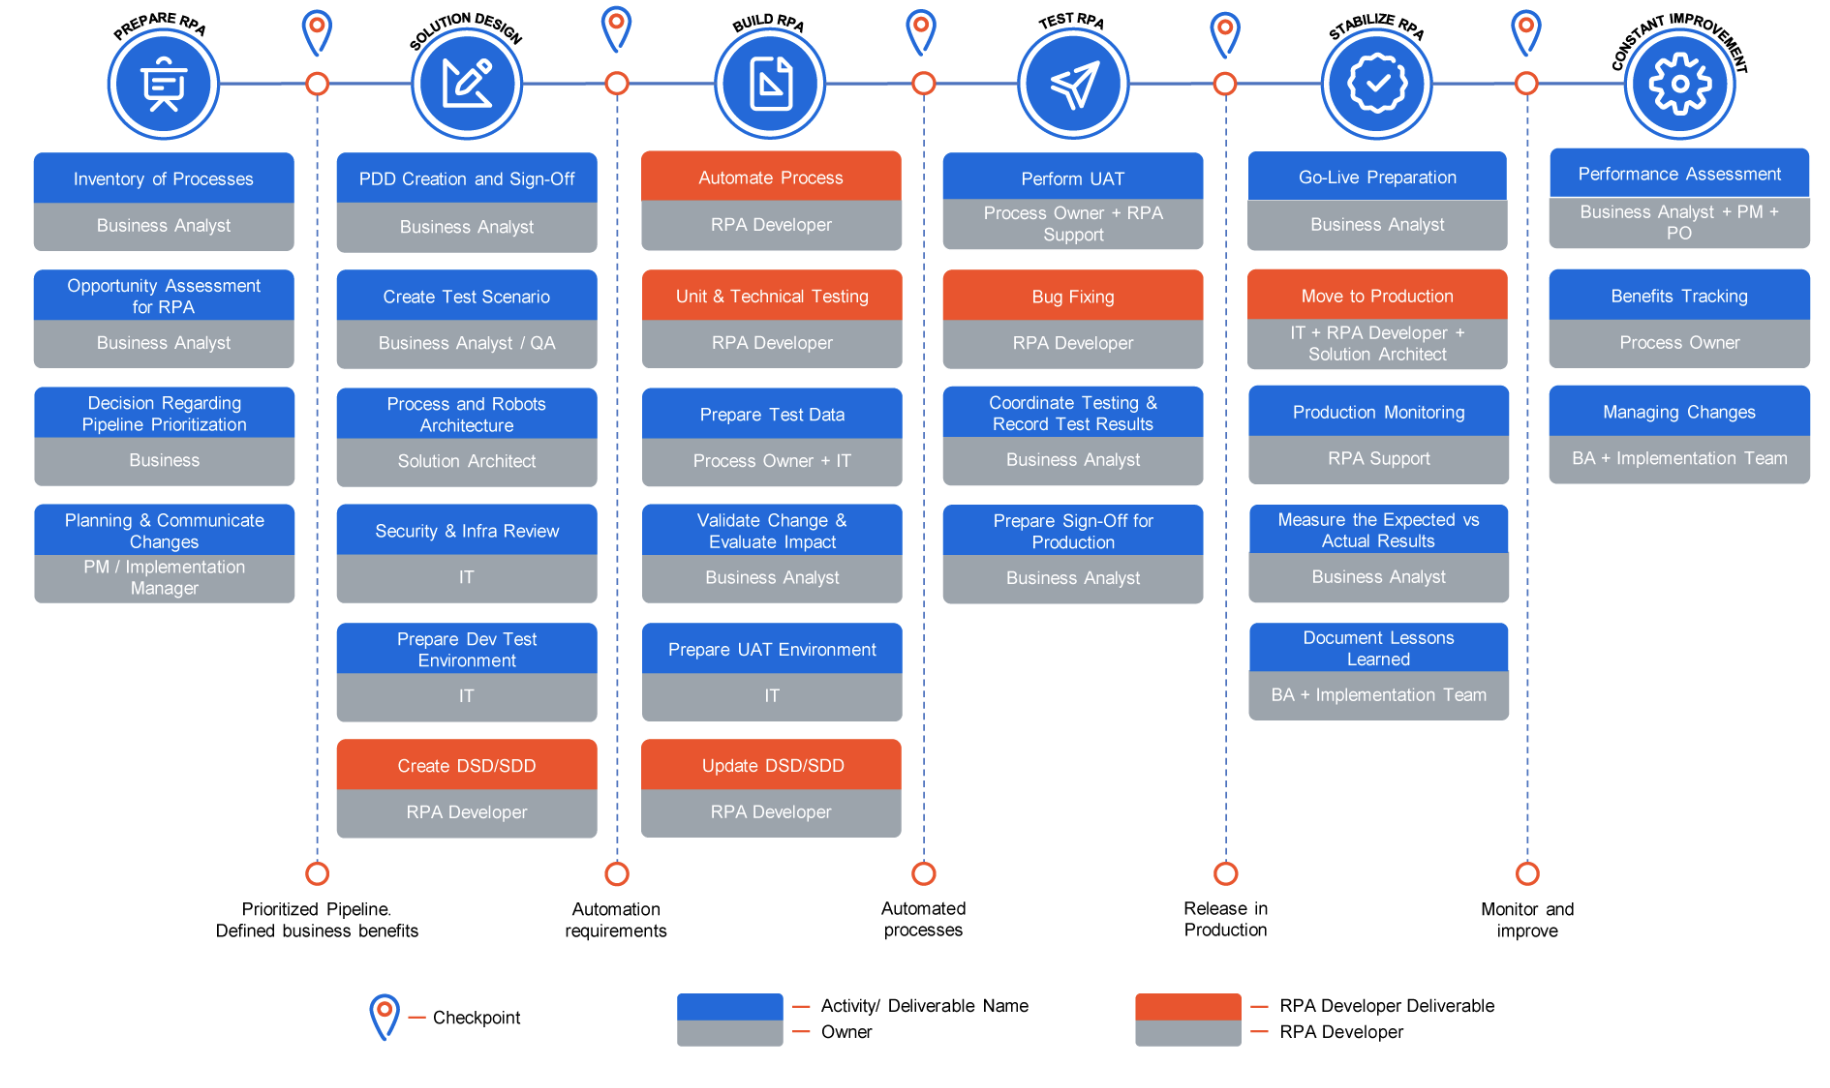
\includegraphics[scale=0.5]{RPASteps}
	\caption{De stappen die overlopen worden tijdens het uitvoeren van een RPA project. (UiPath Academy, 2019)}
\end{figure}

\section{Programmeren in UiPath Studio}
Om een proces te automatiseren is een kleine hoeveelheid programmeerwerk nodig binnen UiPath. Hiervoor kan beroep gedaan worden op de programmeertalen C\# of VB.NET. Hierbij gelden de algemene regels van programmeren. 

\subsection{Variabelen en Argumenten}
Zo zijn er vele verschillende data types waarbij de meest gebruikte zijn: Int32, Long en Double als Numeric values. Booleans voor true of false waarden. Strings voor tekst. DateTime en TimeSpan om te werken met datums en tijd. Ook collections zoals arrays of lists en DataTable voor tabelstructuren worden ondersteund. Een speciaal veel voorkomend datatype is GenericValue, het type gebruikt wanneer er niet geweten is wat er nu exact in de variabele gaat zitten.

Naast variabelen kent UiPath Studio ook argumenten. Argumenten worden ook gebruikt om data in op te slaan en hebben dezelfde datatypes. Het grote verschil met variabelen zit in de scope. Argumenten kunnen gebruikt worden om data tussen verschillende workflows door te geven. Hiervoor gebruiken ze speciale in/uit directionele eigenschappen.

\subsection{Control Flow}
Structuren zoals if/else, while en for worden ondersteund in zowel de flowchart als de sequence.

\subsubsection{Sequence}
In een sequence flow volgen de stappen elkaar op in een duidelijke volgorde. Ze zijn makkelijker te lezen dan flowcharts, gebruiken minder beslissingspunten en zijn dus geschikt voor lineaire workflows.

\subsubsection{Flowchart}
In een flowchart zijn de activiteiten moeilijk te lezen maar de flow tussen deze verschillende activiteiten is makkelijk af te lezen. Hierbij wordt vaak gebruik gemaakt van beslissingspunten.

\subsection{RPA specifieke interacties}
\subsubsection{Excel}
RPA heeft een aantal activiteiten die gespecialiseerd zijn om te werken met spreadsheets zoals Excel. Hierbij wordt een onderscheid gemaakt tussen Excel (.xlsx) en andere formaten zoals (.xls, .csv). De grote verschillen tussen de 2 is dat voor te werken met .xlsx, Excel geïnstalleerd moet zijn op de computer waarop de RPA robot draait, voor de andere extensies kan een ander spreadsheet programma gebruikt worden. Het voordeel echter van te werken met Excel is dat dit in de achtergrond kan uitgevoerd worden.

\subsubsection{UI Interacties}
Interacties met een UI kunnen opgedeeld worden in 2 categorieën: input en output. Input acties gaan over klikken, hoveren en typen in UI elementen. Output acties gaan data ophalen uit een UI element.

De input categorie kan nog verder opgedeeld worden in 3 soorten:
\begin{itemize}
	\item Default: deze manier werkt via echt clicks en typen. Hierdoor is het vrij traag en je mag niet interageren met de muis of het keyboard tijdens dat het proces loopt. Het is wel 100\% ondersteund door elk platform. 
	\item Window Messages: speelt window messages af die verstuurd worden naar de applicatie wanneer keyboard of muis gebruikt worden. Hierdoor is het invullen van tekst direct. Deze methode werkt even snel als de default methode maar kan ook uitgevoerd worden op de achtergrond.
	\item Simulaties: maakt gebruik van de achterliggende A Programming Interface (API) om taken op het systeem uit te voeren. Dit zorgt ervoor dat simulaties snel uitgevoerd kunnen worden op de achtergrond. Het wordt wel minder ondersteund.
\end{itemize}

Ook output interacties kunnen verder opgedeeld worden:
\begin{itemize}
	\item Full-Text: dit is de standaard methode om data op te halen. Het is de meest accurate manier en is goed genoeg voor 90\% van de gevallen en kan zelfs verborgen tekst zien.
	\item Native: maakt gebruik van de Graphics Design Interface (GDI), een microsoft API die grafische objecten voorstelt. Het kan alleen gebruikt worden met applicaties die GDI ondersteunen. Dit gaat vrij traag maar kan wel buiten tekst ook posities gaan ophalen.
	\item OCR: Optical Character Recognition is de enige manier die werkt via een virtuele omgeving waarbinnen het tekst probeert te lezen van een foto die gemaakt wordt. Dit is veruit de traagst en minst accurate manier.
\end{itemize}

Om te weten over welk UI elementen het gaat bij bijvoorbeeld het klikken op een bepaalde button of het invoeren van tekst in een bepaald tekstvak, genereert RPA voor elk element een selector. Een selector is een uniek pad dat RPA laat weten over welk element het gaat. Hierdoor kan RPA dit element altijd terug vinden, zelfs al zijn er kleine UI wijzigingen. De selector zelf wordt opgeslagen als XML. Een voorbeeld selector: `<webctrl parentid=‘slide-list-container’ tag=‘A’ aaname=‘Details’ class=‘btn-dwnl’ />` waarbij webctrl de tag is die zegt over welke soort applicatie het gaat. Andere tags zijn bijvoorbeeld html of java. De attributen geven extra informatie aan deze tag. De attributen op dit voorbeeld zijn parentid, tag, aaname en class.

Er zijn 2 soorten selectors, volledig en partieel. Bij een volledige selector wordt zowel het pad naar de ouder als naar het element zelf bijgehouden. Bij partiële selectors worden deze paden niet bijgehouden, hieruit volgt dat ze altijd in een container moeten gebruikt worden, anders zijn ze niet te herkennen.

\subsection{Project layout}
Het is belangrijk om de correcte layout van het project te kiezen gebaseerd op het proces dat geautomatiseerd moet worden. Er zijn 3 grote layouts:
\begin{itemize}
	\item Sequence: gebruikt wanneer er een duidelijke opvolging van stappen zonder al te veel condities (if/else en switch activiteiten). Meestal worden ze gebruikt om delen uit te werken en te nesten in hogere logica van Flowcharts of State Machines. Ze zijn makkelijk te lezen maar te veel condities zorgt ervoor dat ze moeilijk te lezen worden. Ze zijn niet geschikt voor een continue flow.
	\item Flowchart: gebruikt voor een meer complexe flow waar meerdere condities tot verschillende paden leidt. Ze zijn makkelijk te lezen en kunnen gebruikt worden voor een continue flow.
	\item State Machine: is een abstract concept, bestaande uit een eindig aantal voorgedefinieerde statussen en transities tussen deze statussen. Op elk punt kan de software zich slechts in 1 status bevinden. Ze worden gebruikt voor complexe continue workflows uit te werken. Door de flexibiliteit en de simpele transities tussen de statussen kunnen gemakkelijk alle 'edge cases' mee opgenomen worden in het proces. Het nadeel hieraan verbonden is dat het langer duurt om een state machine te implementeren juist vanwege de complexiteit. Ook zal moeten besproken worden hoe het proces opgesplitst moet worden in verschillende statussen en transities.
\end{itemize}

Het beste is om het hele automatiseringsproject op te splitsen in kleinere, minder gecompliceerde stukken. Er zijn 3 factoren waarmee rekening moet gehouden worden bij het splitsen van workflows: de applicatie die wordt geautomatiseerd, het doel van één bewerking en de lengte van elke workflow. Bij het splitsen moeten argumenten gebruikt worden in plaats van variabelen, door hun bredere scope.

\subsubsection{Project hergebruiken}
het opslaan en hergebruiken van componenten in afzonderlijke projecten gebeurt via procesbibliotheken. Dit zijn pakketten die een of meer herbruikbare componenten bevatten.

\subsubsection{Teams}
Een RPA project kan perfect gedeeld worden binnen een team door gebruik te maken van een version control systeem zoals Git of Azure Devops Server (TFS).

\subsection{Exceptions}
Exceptions  kunnen optreden tijdens de uitvoering van een workflow. Er zijn twee manieren om met deze uitzonderingen om te gaan. Op activiteitenniveau met try / catch-blokken en retry-scope activiteiten of op globaal niveau, met behulp van de global exceptionhandler.

Om te weten op welk niveau uitzonderingen moeten worden afgehandeld, moet beslist worden welk type exception wordt gegooid. Er zijn 2 types van uitzonderingen: applicatie excepties die fouten beschrijven op een technisch niveau of een business exceptie die een fout beschrijft in het feit dat bepaalde data die cruciaal is voor het automatiseren van een proces, incompleet of afwezig is en dus faalt een business regel. Identificeren welke exceptie gegooid wordt is belangrijk om te weten of een simpele try/catch of retry scope genoeg is om het probleem te kunnen oplossen of niet.

\subsubsection{Error vs Exception}
Fouten zijn gebeurtenissen waar een bepaald programma niet mee om kan gaan, zoals syntaxisfouten, gebruikersfouten en programmeerfouten.
Uitzonderingen zijn gebeurtenissen die door het programma worden herkend, gecategoriseerd en afgehandeld. Enkele veel voorkomende uitzonderingen zijn: NullReferenceException, IndouxOutOfRangeException, ArgumentException en SelectorNotFoundException.

Business rule exceptions staan los van de systeem excepties. Ze worden niet gegooid onder de System.Exception class en moeten elk specifiek afgehandeld worden.

\subsubsection{Try/Catch}
De try / catch-activiteit werkt net als bij programmeren. De activiteit die mogelijks mislukt, wordt in het try-blok geplaatst. Het catch-blok is waar naartoe gegaan wordt als een uitzondering optreedt en waar de exceptie afgehandeld wordt. Het finally-blok wordt altijd uitgevoerd na de try / catch.

\subsubsection{Retry Scope}
De retry-scope is een activiteit die één bepaalde activiteit of reeks activiteiten opnieuw probeert totdat het opgegeven aantal pogingen is bereikt, de toepassing geen uitzondering meer geeft of totdat aan de voorwaarde voor opnieuw proberen is voldaan.

\subsubsection{Global Exception Handler}
De Global Exception Handler is een type workflow dat is ontworpen om het gedrag te bepalen bij een uitvoeringsfout op projectniveau. Dit is de reden dat er slechts één globale handler per automatiseringsproject kan worden ingesteld. Alleen niet opgevangen uitzonderingen bereiken de uitzonderingshandler: als er een uitzondering optreedt in een try / catch-activiteit en deze met succes wordt gevangen en binnen het catch-blok wordt behandeld, zal deze de globale uitzonderingshandler niet bereiken.

\subsection{Debugger}
UiPath heeft een ingebouwde debugger om de workflows en sequenties stap voor stap te doorlopen en zo het project te debuggen.
